\section{Deep Learning}
\subsection{Supervised Learning with Gradient Descent}
Machine learning is about solving problems we do not know how to solve directly.
Rather, we perform some kind of statistical inference.
In supervised machine learning, we are trying to learn a mapping from inputs to outputs, for example between the pixels of an image and the classification of that image.
Neural networks are a type of mapping known as a \textit{parametric} model.
I will outline here the general procedure for training such a model before detailing the specifics of neural networks themselves.

To first step to learning this mapping is to obtain some \(\{x_i \in \R^n, \ y_i \in \R^m\}_{i=1}^N\) data points to learn from, called the training data.
Then, we pick some functional representation, such as \(y = wx + b\), where \(w \in \R^{m \times n}, b \in \R^m\); meaning we approximate the true mapping as a linear function.
We will attempt to learn from the data the parameters \(w, b\) that specify the exact linear function that solves the problem.
Note, \(\theta\) is often used as a single variable to denote all the parameters.
We will call our linear function given those parameters \(f_\theta : R^n \rightarrow R^m\).
It is often referred to as the model, or the network in the case of neural networks.

To conduct learning, we need a performance metric for our function and a method to optimise the parameters with respect to that metric. The performance metric is often referred to as a loss function, cost function, or error function; and evaluates how 'good' the parameters are using the training data. We denote this loss function, \(L_D : \Theta \rightarrow \R^+\), where \(\Theta\) is the set of all possible parameters and \(D\) is the training data. A common loss function is of the structure:

\begin{equation*}
    L_D(\theta) = \frac{1}{N}\sum_{i=1}^N l(f_\theta(x_i),\, y_i)
\end{equation*}

where \(l : \R^m\times\R^m \rightarrow \R^+\) measures the `loss' between the true outputs, known as the targets, and what \(f_{\theta}\) produced, for that specific data point. This could be the square-error loss \(l(o, t) = (o-t)^2\), for example.

Thus, the original problem has been reduced into an optimisation problem. Specifically, the objective is to minimise \(L_D\) with respect to \(\theta\).

We can do this using gradient descent \cite{Cauchy1847}. This is an iterative method that follows the line of steepest descent (the gradient) down the slope in small increments, often likened to placing a ball on the loss surface and watching it roll down to the minimum point. Formally, the procedure is to initialise our parameters to some \(\theta_0\) before iteratively applying the following update rule until we are satisfied with our parameters:

\begin{equation*}
    \theta_{k+1} = \theta_k + \eta((\nabla L_D)(\theta_k))^\top
\end{equation*}

Where \(\nabla L_D\) is the Jacobian matrix of the loss with respect to the parameters, and \(\eta\) is a small, positive number known as the learning rate. Given sufficiently small \(\eta\), the sequence \(L_D(\theta_0) \,\geq\, L_D(\theta_1), \,\geq\, L_D(\theta_2), \,\geq\, \ldots\) must converge to a local minimum of \(L_D\). 

\subsection{Mini-Batch Stochastic Gradient Descent}
Attempting to use gradient descent exactly as described above leads to some issues in the real-world. Firstly, every single weight update step requires iterating over the entire dataset to evaluate the loss. Real world datasets are very large, for example the ImageNet Large Scale Visual Recognition Challenge (ILSVRC) Object Localisation dataset has over 1.2 million images \cite{ILSVRC15}. Iterating over this entire dataset for a single weight update would be prohibitively slow. Secondly, recall gradient descent is only guaranteed to converge to the \textit{local} minima. For our simple example, the loss function is convex, so this is not a problem. However, to model complex real world problems, we need more expressive functional representations that can model highly complex non-liearities, leading to a non-convex loss. As an example, the loss surface of the VGG-56 \footnote{VGGNets are a popular neural network architecture for computer vision tasks. A VGGNet won the object localisation task of the ILSVRC in 2014.} network \cite{Simonyan2014} is visualised in Figure \ref{fig:2-vgg-loss}. Note it has many narrow local minima for gradient descent to get stuck in.

\begin{figure}[htb]
    \centering
    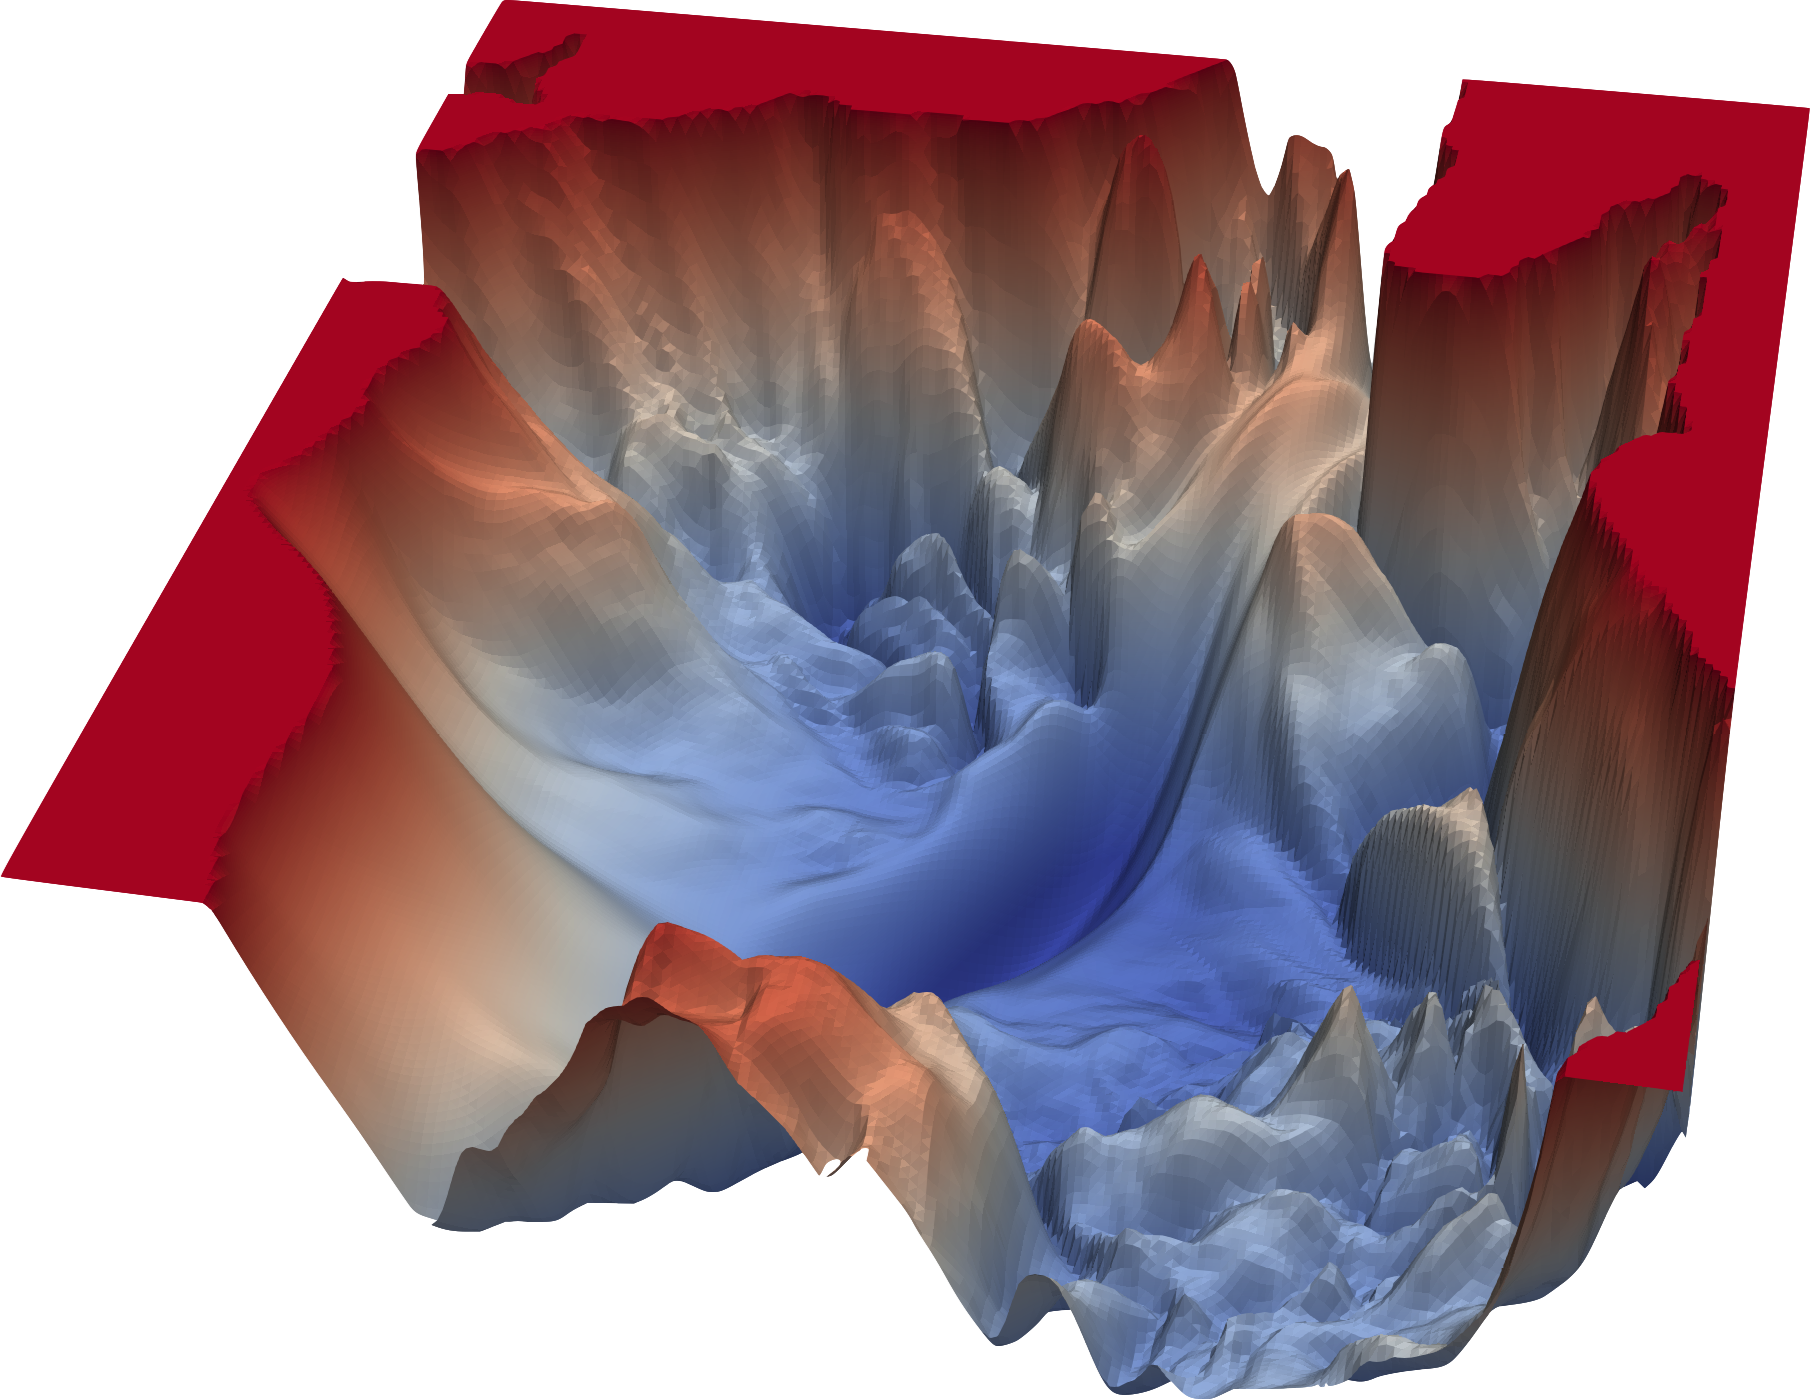
\includegraphics[width=0.7\linewidth]{vgg_56_loss.png}
    \caption{Visualisation of the loss function of VGG-56 \cite{Li2018}.}
    \label{fig:2-vgg-loss}
\end{figure}

To work around these problems, stochastic gradient descent (SGD) is used \cite{Bottou2018}. Rather than updating the parameters by computing the loss over the entire dataset, only a small `mini-batch' is used for one update step. This approximates true gradient descent and takes more steps to converge, but each step is now actually computable. Moreover, it means that on every update we are actually descending a different loss curve, \(L_B\), defined by the mini-batch \(B\subseteq D\) we are working on, as opposed to always using the same loss curve \(L_D\) that sums over all of the data. To see why this is beneficial, consider when after an update we have reached the local minima for that loss, but not the true global minima. On the next update, we are descending a different loss curve that likely does not have that exact local minima too, so we can ‘fall through it’ and continue towards the global minima.

\subsection*{A Note on Stochastic Gradient Descent in Practice}
In conclusion, I have outlined the SGD process used to train models in machine learning, which will be applied to neural networks in the next section and made memory-efficient in the remainder of this thesis.

It should be noted, however, that even SGD is not actually good enough by itself.
Much research goes into improving the optimisation methods of machine learning.
Commonly used techniques include dropout \cite{Srivastava2014}, L1/L2 regularisation \cite{Anders1992-weight-decay, Ng2004}, momentum \cite{Sutskever2013}, and Adam Optimisation \cite{Kingma2015-adam}.

None of these methods significantly affect the nature of the memory optimisations presented later, so I will not cover them here.

\subsection{Artificial Neural Networks}
We have talked much about how to train a model, but have so far used a simple linear one.
I will now introduce neural networks.

The problems being solved today, such as computer vision tasks, are extremely difficult.
In these tasks, a simple linear mapping cannot sufficiently express the intricacies of the real underlying mapping being approximated.



% \begin{itemize}
%     \item we have talked much about how to train a model, but have so far used a simple linear one - what models are actually used today to represent the difficult problems we see being solved with machine learning?
%     \item Functional composition of elementary ops, very expressive (universal approx theorem etc)
%     \item So how to do gradient descent on this? Chain rule to get params at each neuron.
%     \item Backpropagation algo, weight update rules
%     \item For more in-depth explanations of underlying theory of machine learning, why NN functional representation, why gradient descent, why certain loss functions, and how they work together, see (literature)
%     \item From weight update rules, derive computational graph. This underlies most optimisations at it says what the computer must actually do to perform backprop.
%      \item We will look at the implications of this graph on memory in checkpointing section and how to overcome them with checkpointing.
% \end{itemize}
